%&pdflatex
\documentclass[1p]{elsarticle}

\usepackage{lineno,hyperref}
\usepackage{amsmath, amssymb, amscd, amsthm, amsfonts}
\usepackage{mathtools}
\modulolinenumbers[5]

\DeclarePairedDelimiter\ceil{\lceil}{\rceil} \DeclarePairedDelimiter\floor{\lfloor}{\rfloor}

\newtheorem{theorem}{Theorem}
\newtheorem{lemma}[theorem]{Lemma}
\newtheorem{conjecture}[theorem]{Conjecture}
\newtheorem{corollary}[theorem]{Corollary}
\newtheorem{example}[theorem]{Example}

\journal{Discrete Applied Mathematics}

\bibliographystyle{elsarticle-num}

\begin{document}
	
	\begin{frontmatter}
		
		\title{On cartesian product and computation complexity of zombies and survivors game}
		
		
		%% or include affiliations in footnotes:
		\author{Ali Keramatipour}
		\ead{alikeramatipour@ut.ac.ir}
		
		\author{Behnam Bahrak\corref{correspondingauthor}}
		\cortext[correspondingauthor]{Corresponding author}
		\ead{bahrak@ut.ac.ir}
		
		\address{School of Electrical and Computer Engineering, College of Engineering, University of Tehran, Tehran, Iran}
		
		\begin{abstract}
		{\it Zombies and Survivors} is a variant of the pursuit-evasion game {\it Cops and Robbers}, with the difference
		that zombies must always move closer to one of their closest survivors. The game is played on a simple graph by
		two players. Th goal of the zombies is to catch the survivors while survivors' objective is to avoid being
		captured. The zombie number of $G$, denoted as $z(G)$, is the minimum number of zombies required to capture a
		single survivor on $G$, no matter what moves survivor makes. In this paper, we prove a conjecture by Fitzpatrick
		et al.\cite{Fitz16} about the zombie number of the Cartesian product of two graphs. This result provides a new
		proof for $z(Q_n) = \ceil*{\frac{2n}{3}}$. We also introduce a new problem regarding {\it capture time} in
		Cartesian product of two graphs. At last, we study computational complexity of zombie number of a graph G, with
		and without a limited capture time.
		\end{abstract}
		
		\begin{keyword}
			Cartesian Product of Graphs\sep Zombie Number\sep NP-Hard
		\end{keyword}
		
	\end{frontmatter}
	
\section{Introduction}\label{section-introduction}

The {\it Zombies and Survivors} game is played on a simple graph by two players. The deterministic version of this game
\cite{Fitz16} is played as follows (note that we only consider the game with a single survivor). Initially, the zombie
player chooses a number $z$ and places $z$ zombies on the graph vertices. Then the survivor player chooses one single
vertex which is the survivor's initial position. Starting with the zombie player, on each player's turn, survivor player
either moves to an adjacent vertex or stays at his current location, while zombie player must move each zombie to one of
its adjacent vertices so that they get closer to the survivor. Here lies the difference between {\it Zombies and
Survivor} and {\it Cops and Robber(s)} games, as in {\it Cops and Robber(s)} cops should not necessarily get closer to
the robber(s), they can either hold their current position, get closer, or further away from the robber(s). Although
zombies are not as intelligent as robbers, they can still choose their path intelligently between the shortest paths.
If any zombie and the survivor ever occupy the same vertex, the survivor is captured and the zombie player wins. The
zombie number of a graph $G$, denoted as $z(G)$, is the minimum number of zombies required so that the zombie player can
always capture the survivor, no matter how survivor moves.

The Cartesian product $G \square H$ of two graphs $G$ and $H$, is a graph with vertex set of $V(G) \times V(H)$, where
vertices $(u_1 , u_2)$ and $(v_1 , v_2)$ are adjacent if and only if $u_1 = v_1$ and $ \{ u_2 , v_2 \} \in E_{H} $, or
$u_2 = v_2$ and $ \{u_1 , v_1 \} \in E_{G}$ \cite{West02}. Figure \ref{fig:p2} shows an example of the Cartesian product
of two graphs.

Capture time in a game, is the maximum number of moves survivor can avoid being captured, while zombie player has $z$
zombies. If this goes to infinity, a survivor-win play exist.

\begin{figure}[h!]
	\centering
	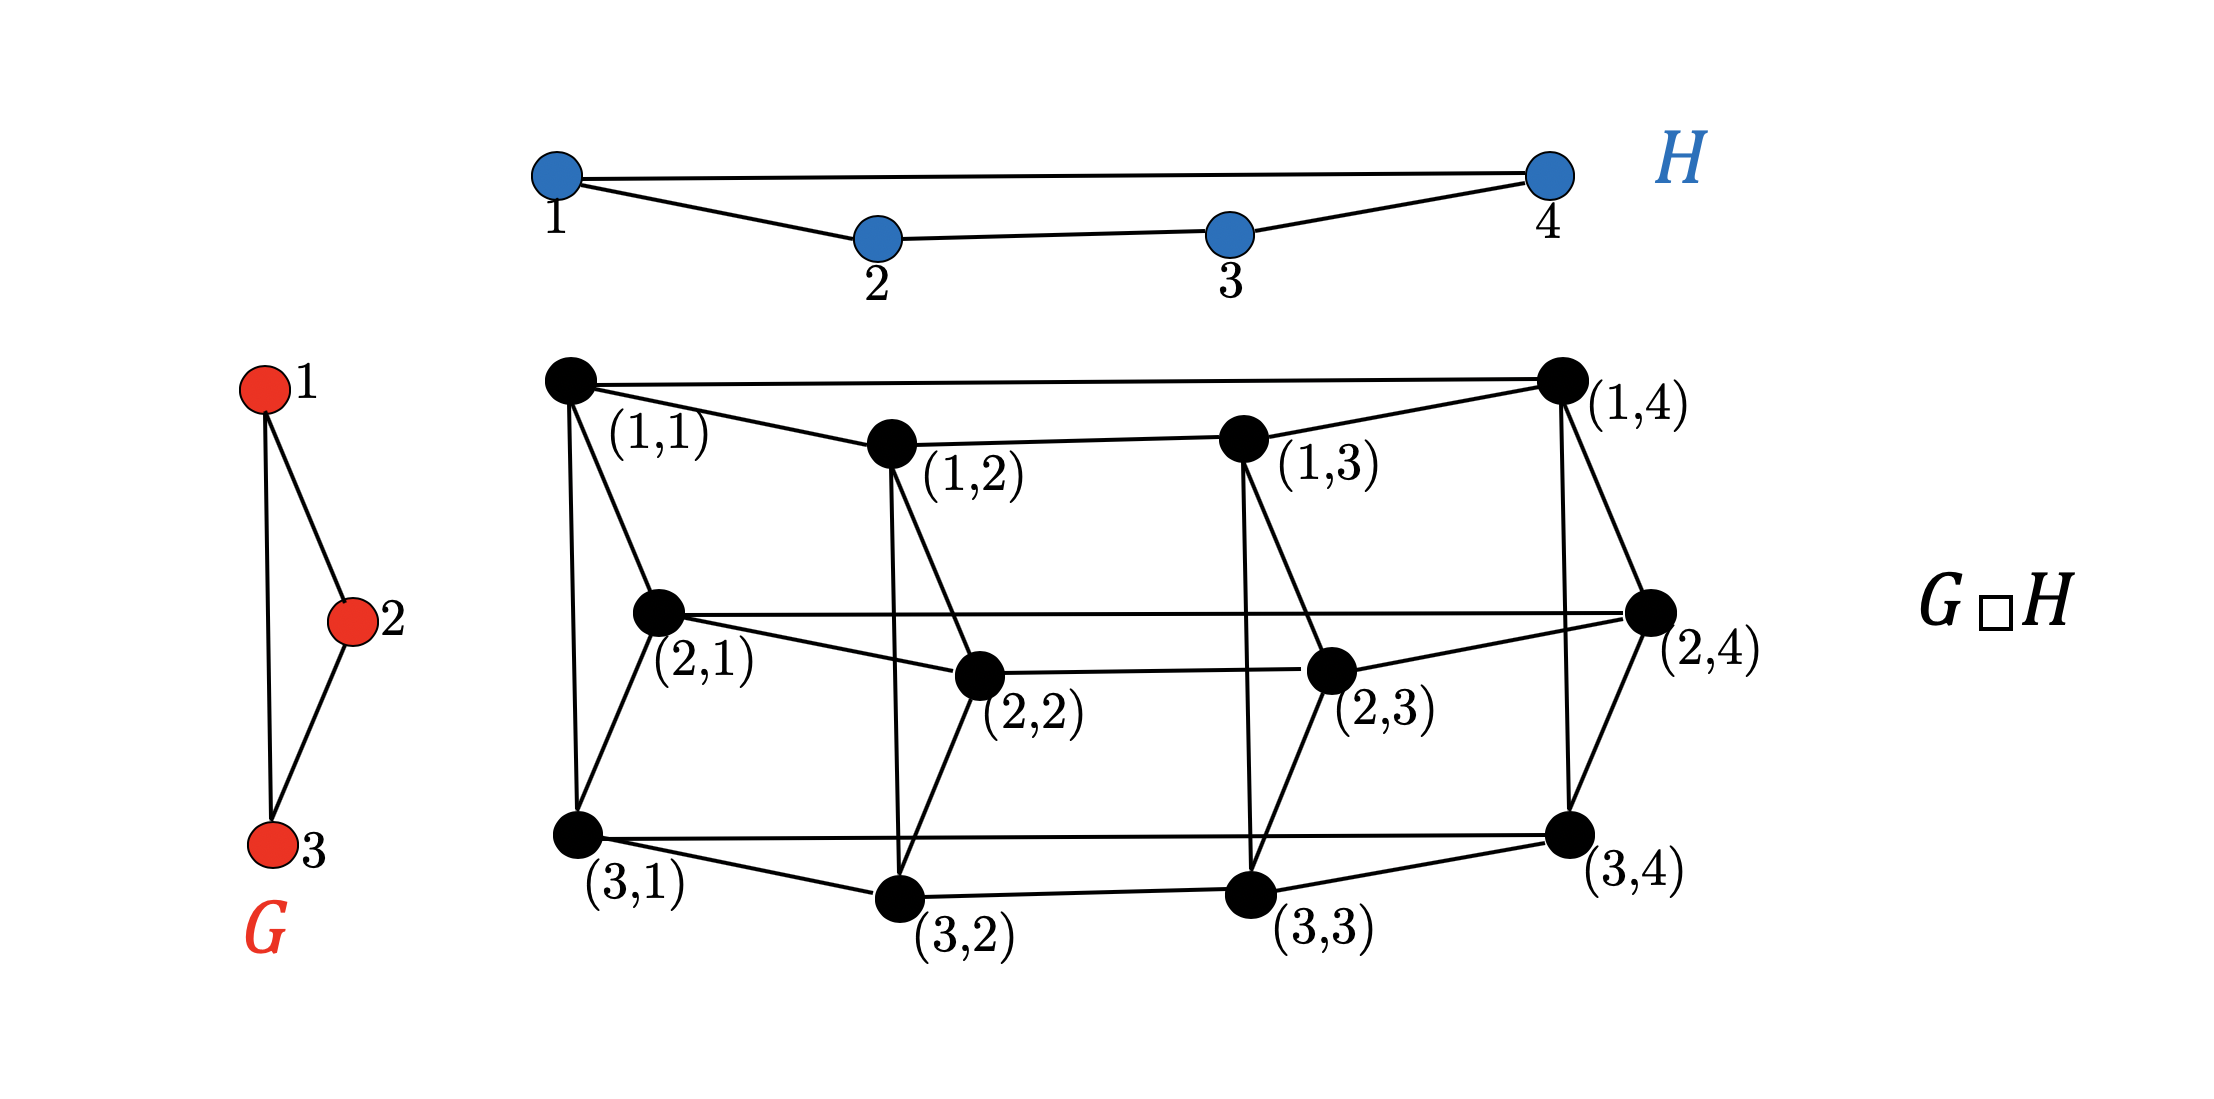
\includegraphics[width=0.9\linewidth]{fig/CpWest.png}
	\caption{$C_3 \square C_4$ an example of a Cartesian product}
	\label{fig:p2}
\end{figure}

Our contributions can be summarized as follows:

1) In \cite{Fitz16}, Fitzpatrick et al. conjectured that $z(G \square H) \leq z(G) + z(H)$. We prove this conjecture and
use it to show that $z(Q_n) = \ceil*{\frac{2n}{3}}$. 

2) We introduce a new problem regarding {\it capture time} and prove a new result in Cartesian product of graphs.

3) We introduce a variation of {\it zombies and survivor} game which zombie player must win in a limited number of
moves and prove it belongs to {\it NP-Hard} set of problems.

4) We prove the original {\it zombies and survivor} game belongs to {\it NP-Hard}.


\section{Zombie number of Cartesian product of two graphs}\label{conj-proof}

To prove $z(G \square H) \leq z(G) + z(H)$, we show that $z(G) + z(H)$ zombies are enough for the zombie player to
capture the survivor on $G \square H$.

To explain the proof we first need to define some notations. Assume $H$ and $G$ have $m$ and $n$ vertices,
respectively. 

Define $G_{i}$ as the induced graph by all vertices $(u,v)$ in $G \square H$, where $v=i$. Similarly
$H_{j}$ is defined as the induced graph by vertices $(u,v)$ in $G \square H$, where $u=j$.

In the Cartesian product of $G$ and $H$, each $G_{i}$ $(1 \leq i \leq m)$ is isomorphic to $G$, and each $H_{j}$ $(1
\leq j \leq n)$ is isomorphic to $H$. We name the common vertex between $G_{i}$ and $H_{j}$, $(i,j)$. Also $(x,y)$ is
the vertex where the survivor is located. Figure \ref{fig:p1} illustrates these definitions.

A {\it G-edge} is an edge in one of the $G_{i}$s and an {\it H-edge} is an edge in one of the $H_{j}$s. A {\it G-move}
is a move made on a {\it G-edge}. Similarly, an {\it H-Move} is a move made on an {\it H-edge}. If the survivor decides
to remain in its current vertex, this move is considered both a {\it G-move} and an {\it H-move}. 

$dist_I(j,k)$ is the distance between $j$ and $k$ vertices on a graph $I$. Length of a path $P$ is shown by $len(P)$. 

A $G$-equivalent graph, is defined as a graph where each zombie in vertex $(z_x,z_y)$, in an arbitrary set of zombies,
is placed on $z_x$ vertex and survivor is placed on $x$ vertex. $H$-equivalent is also defined in the same way. 


\begin{figure}[h!]
	
	\centering
	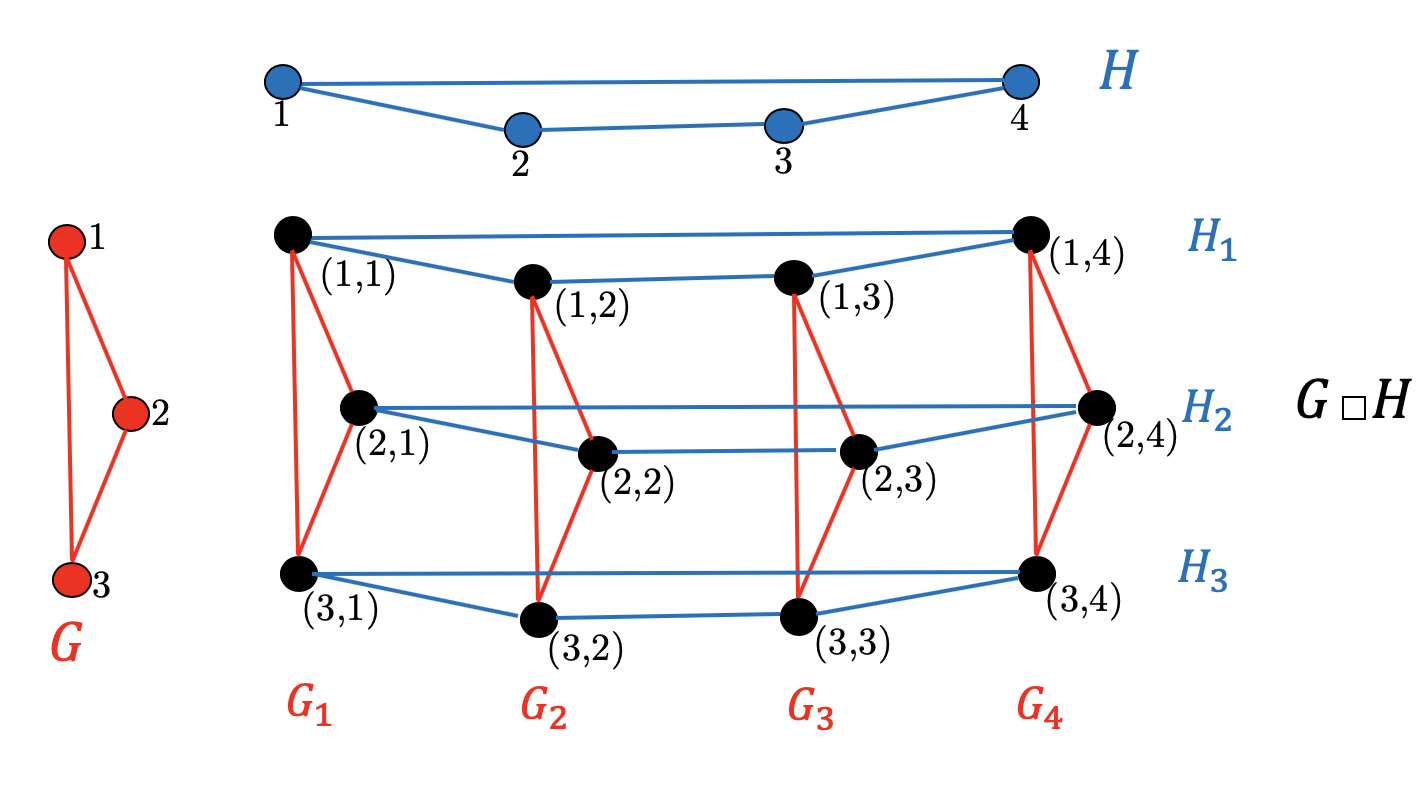
\includegraphics[width=0.9\textwidth]{fig/cp3.png}
	%\includegraphics[width=200pt]{cp.png}
	\caption{$G \square H$, $G_i$s, and $H_i$s.}
	\label{fig:p1}
\end{figure}



\begin{lemma} \label{shortestpathlemma}
	$dist_{G \square H}((x,y),(u,v)) = dist_G(x,u) + dist_H(y,v)$.
\end{lemma}
\begin{proof}
	Since there is a path from $(x,y)$ to $(x,v)$ with length $dist_H(y,v)$ and a path from $(x,v)$ to $(u,v)$ of length
	$dist_G(x,u)$, we only need to prove there can be no path with length less than $dist_G(x,u) + dist_H(y,v)$.
	Suppose not, this path uses some {\it G-move}s and some {\it H-move}s. If a {\it G-move} is followed by an {\it
	H-move} (or vice-versa), then we can swap these moves and still end up in the same vertex. For example if $(u_1,v_1)
	\rightarrow (u_2,v_1) \rightarrow (u_2,v_2)$ is happening, we can do $(u_1,v_1) \rightarrow (u_1,v_2) \rightarrow
	(u_2,v_2)$. Since we can swap each two moves of different type, suppose all {\it G-move}s happen before all {\it
	H-move}s in the shortest path. Since this path has a length less than $dist_G(x,u) + dist_H(y,v)$, we have found a
	path in either $G$ between $x$ and $u$ with length less than $dist_G(x,u)$, or in $H$ between $y$ and $v$ with
	length less than $dist_H(y,v)$, which is a contradiction. Thus the statement holds.
\end{proof}




\begin{theorem}
	$z(G \square H) \leq z(G) + z(H)$.
\end{theorem}

\begin{proof}
	We provide a winning strategy for the Cartesian product of $G$ and $H$ using $z(G)+z(H)$ zombies. First, we place
	$z(G)$ zombies, that have a winning strategy on a single $G$, $G_{z = 1}$ and call them {\it G-zombie}s. We do the
	same for $H_{s = 1}$ and call them {\it H-zombie}s.


	Consider one of the shortest paths between vertices $z$ (the $G$-subgraph shared by {\it G-zombie}s) and $y$ in $H$
	and call it $p_H$. We also define $p_G$ in the same manner between $s$ and $x$.


	On each zombie turn, if $z \neq y$, each {\it G-zombie} will move along the $p_H$ path in its corresponding $H$
	subgraph. According to Lemma \ref{shortestpathlemma}, since zombies' and survivor's equivalents on $H$ are getting
	closer, thus their actual vertices on $G \square H$ are getting closer as well and this move is possible. Since they
	are all moving along similar paths (in their corresponding $H$-subgraphs) they will still share the same
	$G$-subgraph. Now consider when $z = y$, {\it G-zombie}s will play their winning strategy (that they had on a single
	$G$) in this case. This move is also possible since in $G$'s strategy, zombies would get closer to survivor on each
	turn. If $z = y$ and survivor makes an {\it H-move}, {\it G-zombie}s will maintain their positioning by mimicking
	the exact same move on their corresponding $H$. This means for those turns that $z=y$ holds, if we consider the
	$G$-equivalent graph between {\it G-zombie}s and survivor, it is just like a simple game played on a single $G$.
	{\it H-zombie}s will follow the same strategy but in their corresponding environment.
	
	
	Suppose using this strategy $G \square H$ is {\it survivor-win}, then the survivor must either do infinite {\it
	G-move}s or infinite {\it H-move}s. Without loss of generality, suppose the survivor makes infinite {\it H-move}s,
	we prove that this is not possible. After $len(p_G)$ number of {\it H-move}s, {\it H-zombie}s will get to $H_x$. Now for
	each {\it G-move} made by survivor and having zombies chasing him, nothing changes in their $H$-equivalent graph.
	Since the survivor can do infinite {\it H-move}s and prevent being caught, it means that survivor could also avoid
	being caught on a single $H$ which contradicts our assumption.
	
\end{proof}
An example for further understanding can be found at \ref{cartesianProductExample}.

\begin{corollary}
	\label{C3}
	$z(Q_{n}) \leq \ceil*{\frac{2n}{3}}$
\end{corollary}
\begin{proof}
	We prove this by using both induction and the theorem proved above. First note that the Cartesian product of
	hypercube graphs $Q_{m}$ and $Q_{n}$ is equal to $Q_{m+n}$. It is easy to see $z(Q_3) = 2$, $z(Q_2) = 2$, and
	$z(Q_1) = 1$. For $n > 3$, we consider $Q_n$ as the Cartesian product of $Q_3$ and $Q_{n-3}$. Using the induction
	base, we know that $z(Q_{n-3}) \leq \ceil*{\frac{2n - 6}{3}}$. According to the proved conjecture $z(Q_n) \leq
	z(Q_{n-3}) + z(Q_3)$ and $z(Q_{n-3}) \leq \ceil*{\frac{2n - 6}{3}} = \ceil*{\frac{2n}{3}} - 2$, we can see that
	$z(Q_n) \leq \ceil*{\frac{2n}{3}}$.
\end{proof}

It is already proved that at least $\ceil*{\frac{2n}{3}}$ zombies are needed to capture one survivor on graph $Q_n$
(Theorem 16 of \cite{Fitz16}):

\begin{theorem}
	\label{T4}
	For each integer $n \geq 1$, $z(Q_n) \geq \ceil*{\frac{2n}{3}} $.
\end{theorem}

Combining {\it Corollary \ref{C3}} and {\it Theorem \ref{T4}} we can conclude that $z(Q_n) = \ceil*{\frac{2n}{3}}$.
This proves Conjecture 18 from \cite{Fitz16} which is already proved in \cite{Offner19} with a different method. 
	

\section{Capture time and Cartesian product}\label{capturetime}
	Define a new parameter, $ct(G,z)$ (capture time), where $G$ is a graph, and $z$ is an integer.
	
	$ct(G,z)$ is the maximum number of moves that survivor can avoid being caught, assuming that both players choose their best
	strategies. Zombie player will play with $z$ zombies and tries to make this number as least as possible, while
	survivor tries to maximize this.

	Also $diam(G)$ is the length of $G$'s diameter.
	\begin{theorem}
		\label{T5}
		$ct( G \square H, z_G + z_H ) \leq diam(G) + diam(H) + ct(G, z_G) + ct(H, z_H)$
	\end{theorem}
	\begin{proof}
		By having $z_G$ zombies as {\it G-zombie}s and $z_H$ zombies as {\it H-zombie}s, and having them follow the same
		set of moves provided in section \ref{conj-proof}, we show that survivor's {\it G-move}s cannot exceed $diam(H)
		+ ct(G, z_G)$. With the same conclusion, it can be shown that {\it H-move}s cannot exceed $diam(G) + ct(H, z_H)$
		as well.

		After at most first $diam(H)$ {\it G-move}s that survivor makes, $z$ = $y$ holds. Now since for each {\it
		G-move} made from now on by survivor, {\it G-zombie}s can follow their strategy on a $G$ graph, after at most
		$ct(G,z_G)$ {\it G-move}s, survivor will be captured. 
		
		Since each of survivor's moves is either a {\it G-move} or an {\it H-move} or both, total number of moves cannot
		exceed $diam(G) + diam(H) + ct(G, z_G) + ct(H, z_H)$.
	\end{proof}
\section{Limited capture time zombie number Problem is NP-Hard}\label{np-capturetime}

	NP-hardness (non-deterministic polynomial-time hardness) is, in computational complexity theory, the defining
	property of a class of problems that are informally "at least as hard as the hardest problems in NP". A well known
	example of an NP-hard problem is the dominating-set problem in graph theory. A problem is assigned to the NP
	(nondeterministic polynomial time) class if it is solvable in polynomial time by a nondeterministic Turing machine.


	Define $Lcz(G,k)$ as the minimum number of {\it zombies} needed so that zombie player is able to capture the survivor in at
	most $k$ moves. Also $MDS(G)$ is the {\it minimum dominating-set} of graph $G$.
	
	Limited capture time zombie number ($Lcz_k$) problem is defined as below:
	{\newline}
	INSTANCE: Let $G = (V,E)$ be a simple undirected graph. Given graph $G$ and a positive integer $z$.
	{\newline}
	QUESTION: Is $Lcz(G,k) \leq z$ ? In other words, can we capture the survivor after at most $k$ moves using $z$ zombies in graph $G$ ?
	{\newline}
	{\newline}
	The {\it dominating-set} problem is a well-known NP-Hard problem and is defined below:
	{\newline}
	INSTANCE : Given a graph G and an integer z.
	{\newline}
	QUESTION : Does G have a dominating-set of size at most z ?

	\begin{theorem}
		$Lcz_k$ $\in$ NP-Hard
	\end{theorem}
	\begin{proof}
		We prove this by reducing the dominating-set problem, to $Lcz_k$ in polynomial time.

		To have a better understanding, consider the case where $k=1$. For zombie player being able to capture survivor in
		one move, every vertex not occupied by a zombie, should have a zombie neighbor. This is exactly the definition
		of a dominating-set. Dominating set is a subset $D$ of $V(G)$ such that every vertex not in $D$ is adjacent to
		at least one vertex of $D$. This simply shows that $Lcz_1 \in$ NP-Hard 

		Now consider $k$ to be an arbitrary number bigger than 1. We construct a new graph $G'$ from $G$. Suppose $G$
		has $n$ vertices. For each vertex $v \in V(G)$, we add a {\it new} path with $k$ vertices ending in $v$ (as
		shown in figure \ref{fig:p7}), and name each {\it new} vertex $(v,i)$ for $1 \leq i < k$. 
		
		A vertex $v$ is dominated by vertex $u$, if $v = u$ or $v \in N[u]$. A vertex $v$ is dominated by a set $S$, if
		there is a $u \in S$ which dominates $v$.
		
		\begin{figure}[h!]
			\centering
			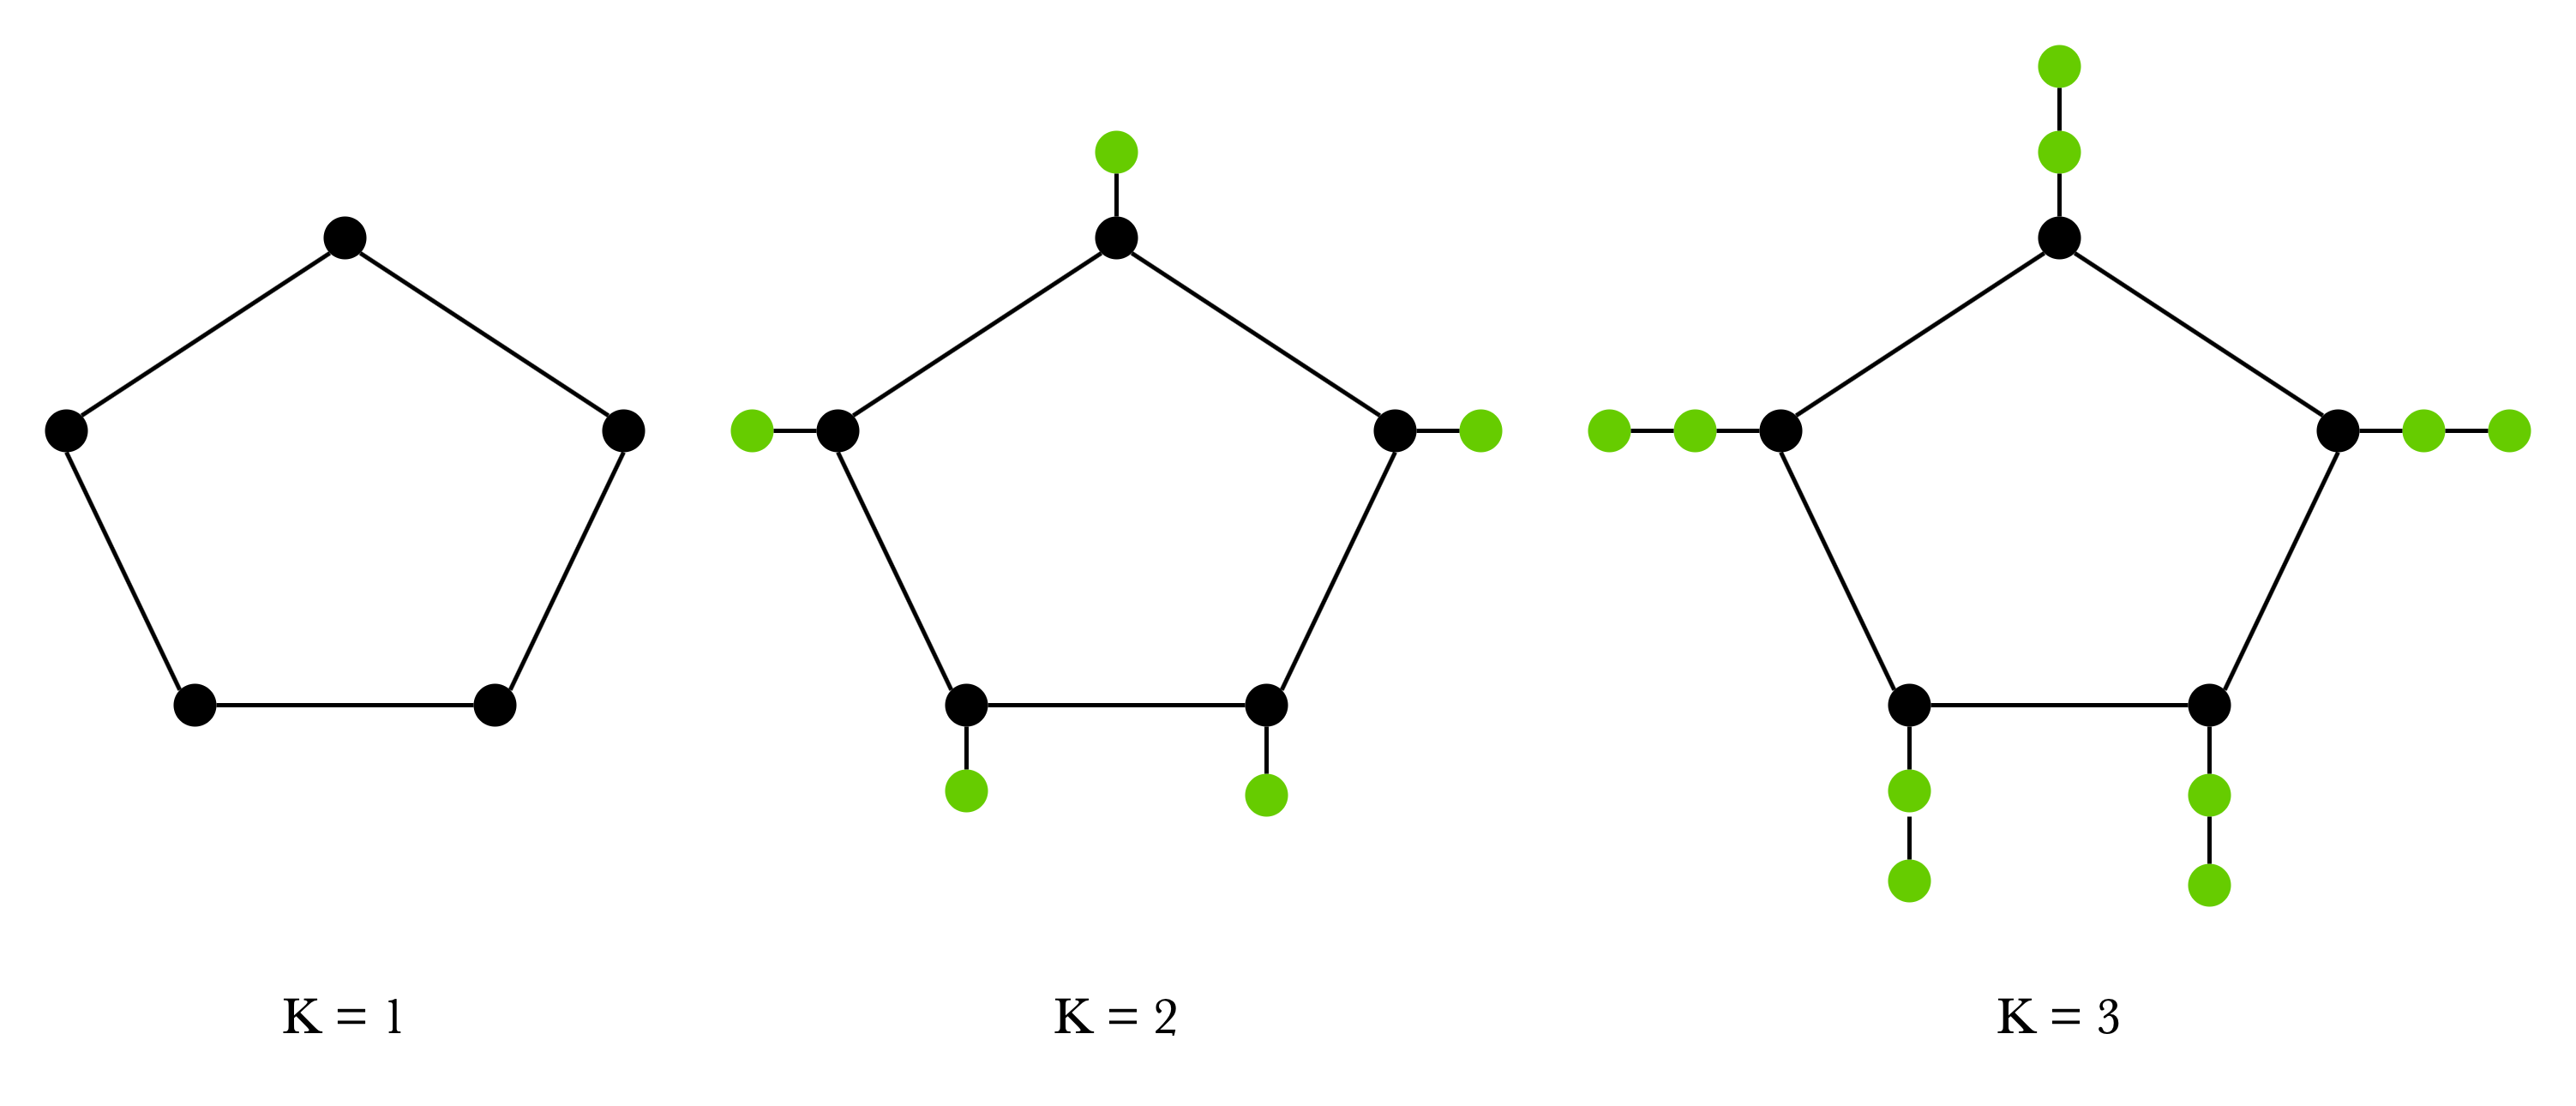
\includegraphics[width=0.9\linewidth]{fig/LCZ.png}
			\caption{$G'$ obtained from $G = C_5$ where for $k = 1,2,3$}
			\label{fig:p7}
		\end{figure}		


		$|V(G')|$ is of $O(nk)$. Thus creating $G'$ can be done in polynomial time. Now we solve $Lcz_k$ on graph $G'$
		and get a number $z$, and a set $S$ of vertices as zombies' initial positions. We now build another set,
		$DS$, on $G$ from set $S$ on $G'$. For each vertex $v \in S$ or $(v,i) \in S$ add $v$ to $DS$. Now suppose $DS$
		is not a dominating-set, thus there is a vertex $u$ not dominated by $DS$. This means there was no zombie on
		vertices $u$ and $(u,i)$ on graph $G'$. By having the survivor on $(u,k-1)$, there is no zombie with distance of
		$k$ or less from him which means that he will not be captured if he doesn't move. Thus, $DS$ must be a
		dominating-set and $ |MDS(G)| \leq |DS| \leq |S| \leq z$.

		Now consider $MDS(G)$. For each vertex $v \in MDS(G)$ place a zombie on vertex $v$ of $G'$. These zombies can
		capture the survivor in at most $k$ moves. To show this consider survivor's initial vertex, if it is an old
		vertex, that is not in the newly added vertices, it can be captured in one move. Now suppose survivor is
		initially on $(u,i)$. Since $u$ is dominated by a zombie, after zombies' move, survivor will be trapped inside
		the $u-path$, and would be captured in at most $k$ moves. Therefore, $z \leq |MDS(G)|$.

		By combining results, $z = |MDS(G)|$. Therefore dominating-set problem is reduced to $Lcz_k$. In the following
		lemma \ref{limit-moves}, we prove this assumption changes nothing.

	\end{proof}

	\begin{lemma}
		\label{limit-moves}
		If survivor can avoid being captured after $(n + 1) * n^2$ moves, he can avoid being captured forever.
	\end{lemma}
	\begin{proof}
		Define $zombieDist$ as sum of the distances between each zombie and survivor. It is not hard to see that after
		each two rounds of play, that is each player has played once, $zombieDist$ won't increase, since zombies are
		always getting closer. Now we show that if $zombieDist$ does not strictly decrease after each player takes turn
		for $n + 1$ times, survivor can avoid being captured forever. Consider the sequence of vertices occupied by
		survivor in $n + 1$ consecutive moves. By pigeonhole principle, one vertex has been seen by survivor at least
		twice. If survivor keeps repeating those moves, he will maintain his distance from zombies and will avoid being
		captured forever.

		Therefore, for a graph $G$ which zombie-player can win, after each $(n + 1)$ move, $zombieDist$ should strictly
		decrease. $zombieDist$ is at most $n^2$, since there is not more than $n$ zombies and each zombie is at distance
		at most $n$ from survivor (this bound can be easily improved). Thus, after $(n + 1) * n^2$ moves, zombies would
		capture the survivor.
	\end{proof}

	By using this lemma, we can see $Lcz_k$ problem for $k > (n + 1) * n^2$ and a graph with $n$ vertices are as same as
	the problem for $Lcz_{(n + 1) * n^2}$, and by solving $Lcz_{(n + 1) * n^2}$ for $G$, we get $z(G)$ as well.


	
	\section{Zombie Number Problem is NP-Hard}\label{np-zombienumber}

	Now define zombie number ($Z$) problem:
	{\newline}
	INSTANCE: Let $G = (V,E)$ be a simple undirected graph. Given graph $G$.
	{\newline}
	QUESTION: Is $z(G) \leq z$ ?

	\begin{theorem}
		$Z \in$ NP-Hard
	\end{theorem}
	\begin{proof}
		We reduce dominating-set problem to $Z$.

		To do this, we add $n$ new complete bipartite graphs, $K_{n,n}$ to $G$. We call the newly obtained graph $H$,
		and recall the $G$-subgraph simply as $G$, and the $i$-th $(1 \leq i \leq n)$ bipartite subgraph as $K_i$.
		$(i,j,b)$ represents the $j$-th vertex in $K_i$'s $b$-th part $(b = 1,2)$ . For each vertex $(i,j,b)$ we connect
		it to vertices $j$ and $N_G[j]$ (neighbors of vertex $j$ in $G$).

		By having zombies on each vertex of $G$'s minimum dominating-set, survivor will be captured on the first move and zombie
		player wins. Thus, $z(H) \leq |MDS(G)|$. Now suppose we have zombies less than $z < |MDS(G)|$. We prove survivor can
		avoid being captured.

		Suppose zombie player has placed his zombies. Since we have $n$ bipartite subgraphs and $z < n$, there is a
		bipartite subgraph, without any zombies in it ($k$-th bipartite graph). Since zombies are not dominating $G$,
		there is a vertex $v$, not dominated by them. We place the survivor on vertex $(k,v,b = 1)$ and survivor has no
		neighbors occupied by a zombie. On each survivor turn, there is a vertex $v$ in $G$ not dominated by a zombie,
		survivor will move to vertex $(k,v,3 - b)$. We prove by following this strategy, he will survive. On zombie
		turn, zombie player has zombies on either $G$ or some $K_i$ $(i \neq k)$ or $K_k$. Initially there is no zombie
		in $K_k$. Now whenever a zombie wants to join $K_k$, first it has to be in $G$ in order to reach $K_k$, as there
		is no connection between $K$-subgraphs. Zombies in $G$ (e.g. at vertex $u$) are at distance 2 from survivor $(u
		\rightarrow (k,u,3 - b) \rightarrow (k,v,b))$, which means after their move all of them should be at one of
		$(k,v,b)$'s neighbors, that is, $v , N[v] $ or, $ (k,1 \leq i \leq n,3 - b)$. Therefore, each zombie joining $K_k$ does
		not share the same partition as survivor's. Survivor now moves to $(k,v,3-b)$ and will be sharing the same
		partition as zombies' in $K_k$. As survivor does not have any neighbors in $G$ or $K_k$ on each zombie player's
		turn, he will not be captured.

		It is now proved that $z(H) = |MDS(G)|$, thus the dominating-set problem is reduced to $Z$.

	\end{proof}

\begin{thebibliography}{999}
	
	\bibitem{Fitz16}
	Fitzpatrick, Shannon L., J. Howell, Margaret-Ellen Messinger, and David A. Pike. "A deterministic version of the
	game of zombies and survivors on graphs." Discrete Applied Mathematics 213 (2016): 1-12.
	\bibitem{Offner19}
	Offner, David, and Kerry Ojakian. "Comparing the power of cops to zombies in pursuit-evasion games." Discrete
	Applied Mathematics (2019).
	\bibitem{West02}
	West, Douglas B. "Introduction to Graph Theory." Prentice hall, (1996).
	\bibitem{reviewer}
	One of our reviewer's notes, Discrete Applied Mathematics, (2020).
\end{thebibliography}

\newpage
\appendix
\section{Cartesian product example} \label{cartesianProductExample}
\begin{example} $z(P_3 \square P_4 ) = 2$
\end{example}

\begin{figure}[h!]
	\centering
	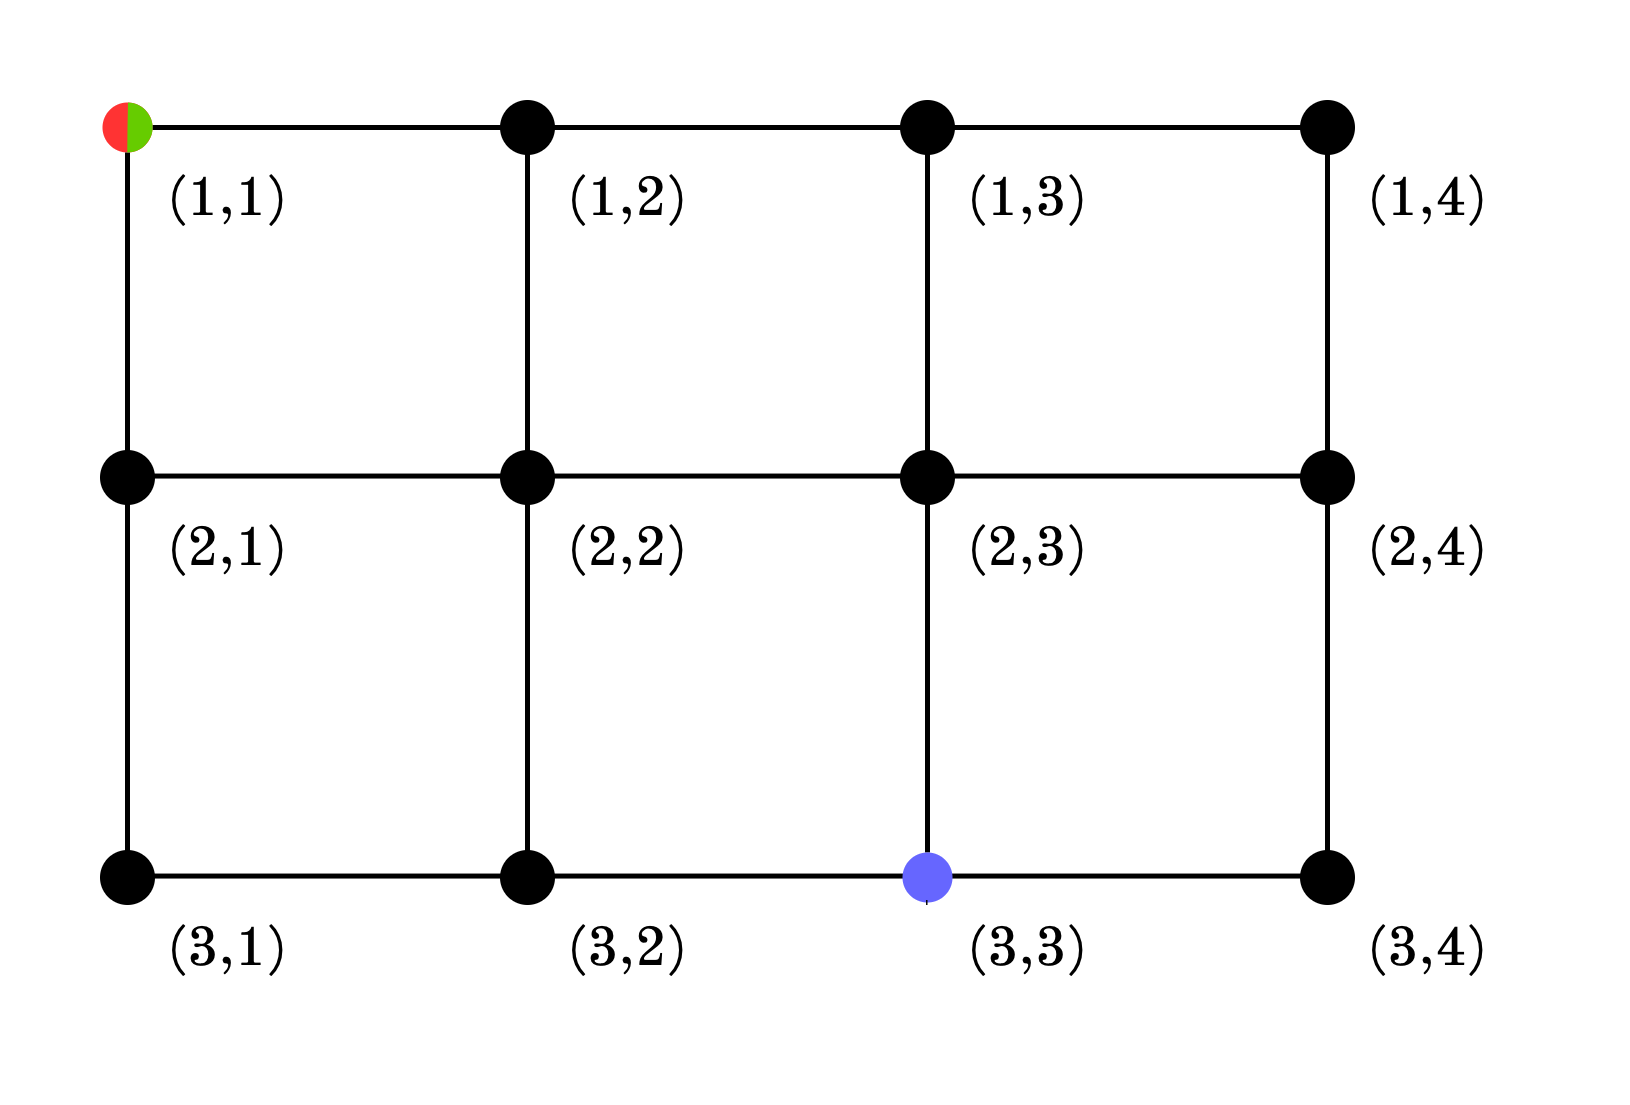
\includegraphics[width=0.5\linewidth]{fig/p34m1.png}
	\caption{$P_3 \square P_4$ and initial vertices}
	\label{fig:p3}
\end{figure}

It is easy to show that $z(P_3) = z(P_4) = 1$. On each of these path graphs, zombie's initial position could be any
vertex of the graph. For this example, we put the {\it G-zombie} and {\it H-zombie} ($G = P_3$ and $H = P_4$) both on
vertex $(1,1)$. We show the survivor with blue color, {\it H-zombie} with red, and {\it G-zombie} with green. {\it
G-zombie} will try to get to the same $G_{i}$ as survivor which is $G_3$ using an {\it H-edge}. {\it H-zombie} will try
to get to $H_3$. See Figure \ref{fig:p4}.

\begin{figure}[h!]
	\centering
	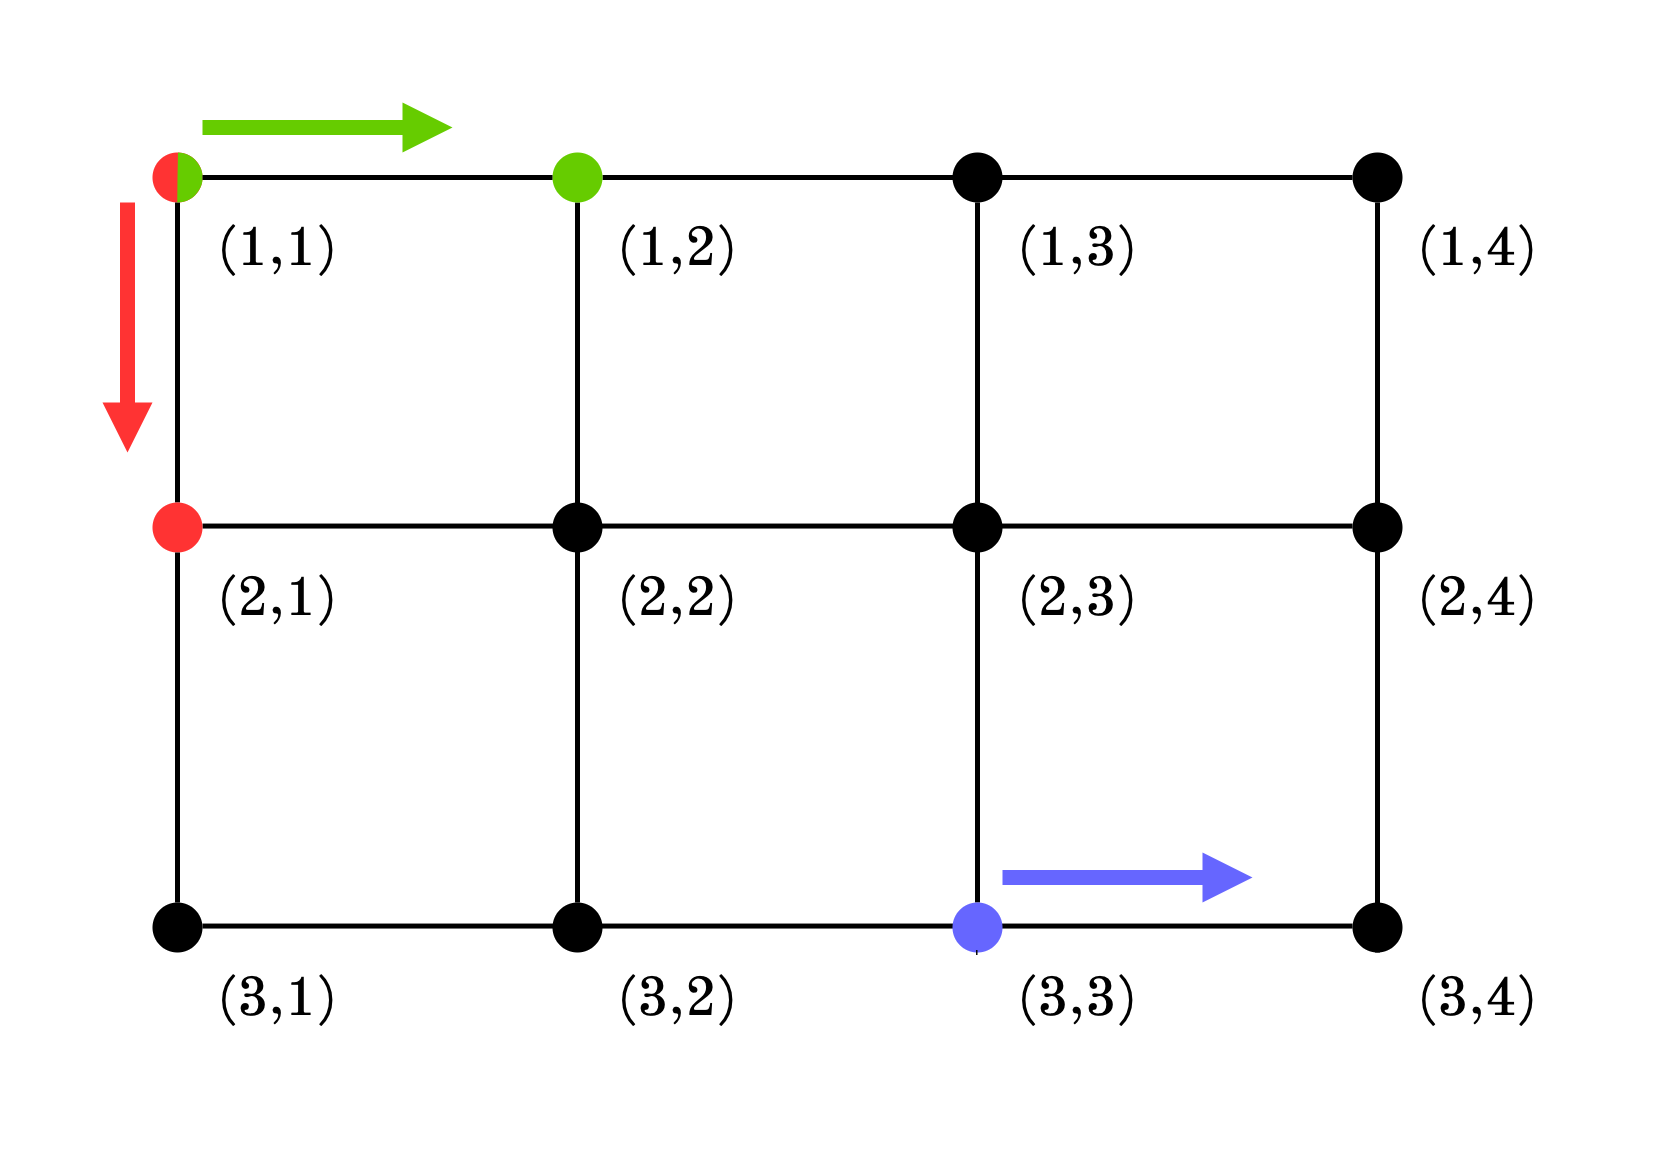
\includegraphics[width=0.5\linewidth]{fig/p34m2.png}
	\caption{First move of players}
	\label{fig:p4}
\end{figure}

After zombies' move the survivor must move. No matter what move he makes, either {\it G-zombie} has made itself closer
to $H_x$ or {\it H-zombie} has made itself closer to $G_y$. In this case, {\it H-zombie} got closer to $H_x$. Since
neither {\it H or G-zombie}s share $H_x$ or $G_y$ with the survivor, they will still try to achieve that (See Figure\ref{fig:p5}).

\begin{figure}[h!]
	\centering
	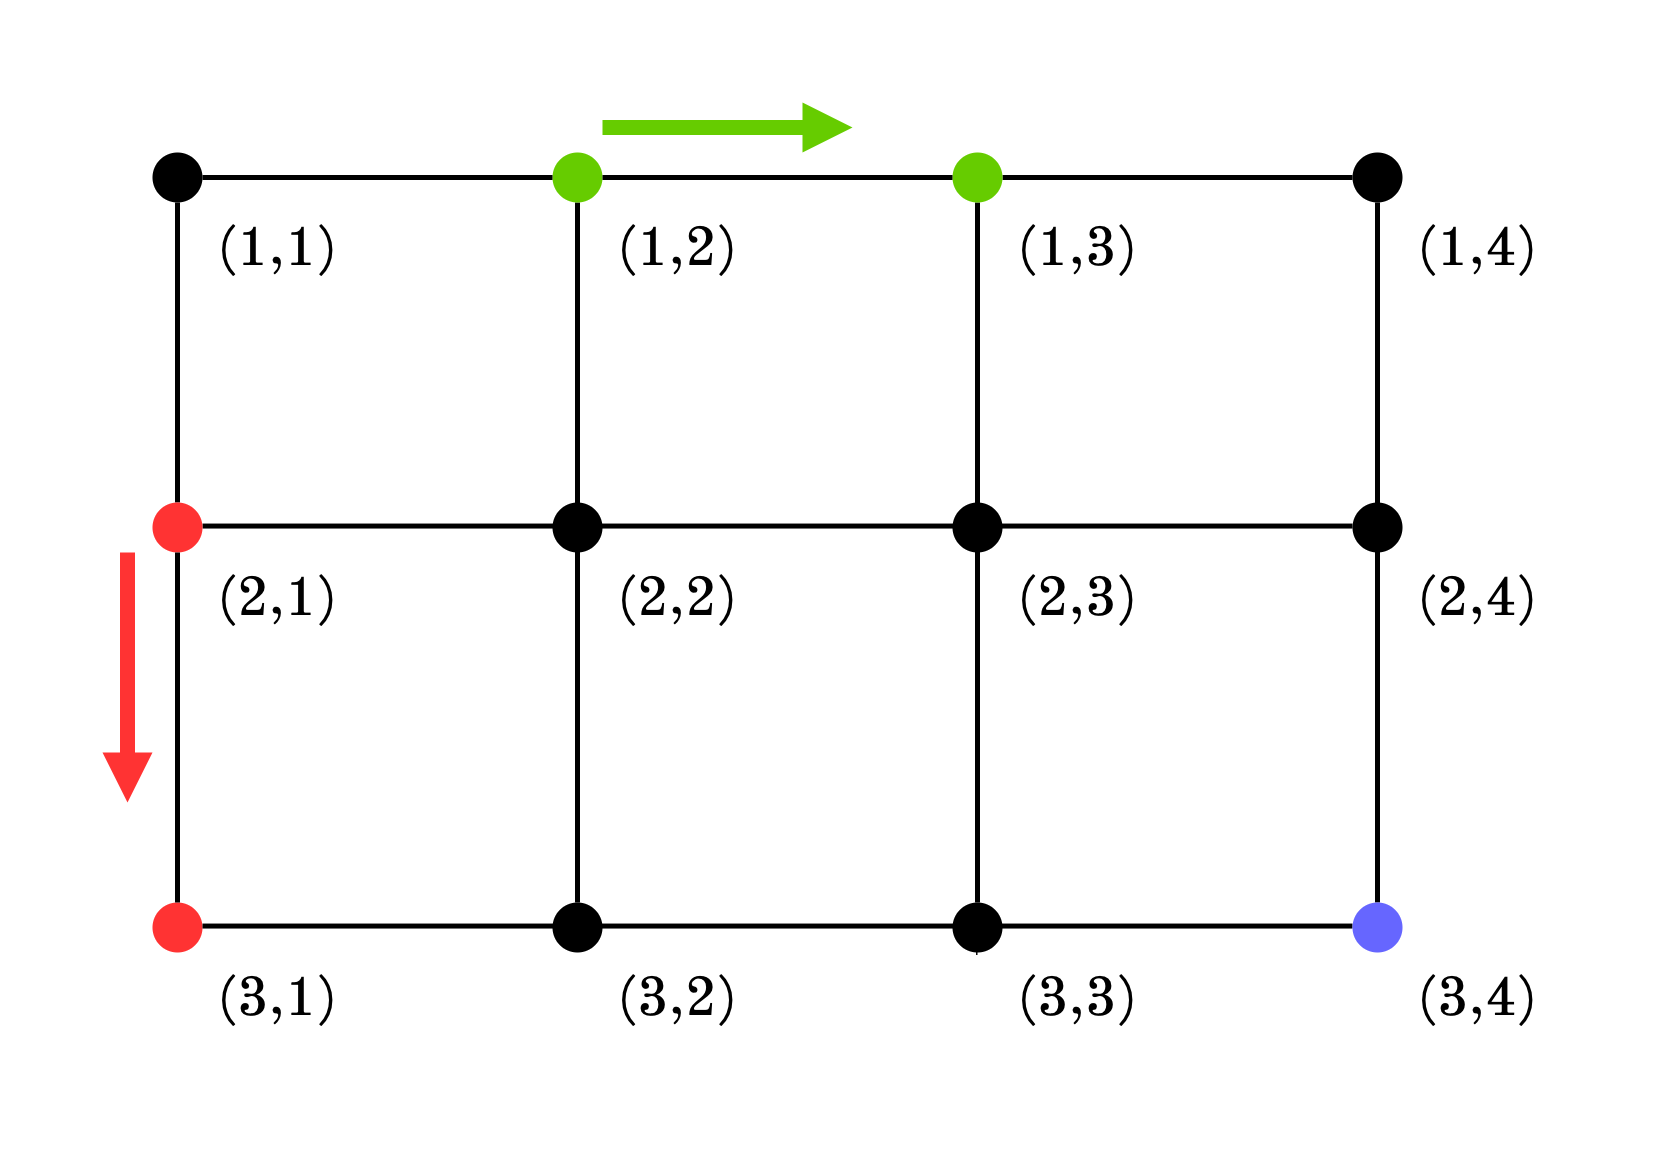
\includegraphics[width=0.5\linewidth]{fig/p34m3.png}
	\caption{Second move made by zombies, third in total}
	\label{fig:p5}
\end{figure}

Now {\it H-zombie} shares the same copy of $H$ as survivor and it is survivor's turn. If survivor moves to another $H_i$,
{\it H-zombie} will mimic the move. If survivor makes an {\it H-move}, {\it H-zombie} will do whatever it did on a
single $H$. This means survivor cannot do infinite {\it H-move}s. Thus for him being able to survive he has to do
infinite {\it G-move}s, which again leads to {\it G-zombie} capturing him. For other moves, you can see
Figure\ref{fig:p6}. We cannot discuss each possible survivor move since they are a lot, but you can still easily apply
the strategy provided above. 

\begin{figure}[h!]
	\centering
	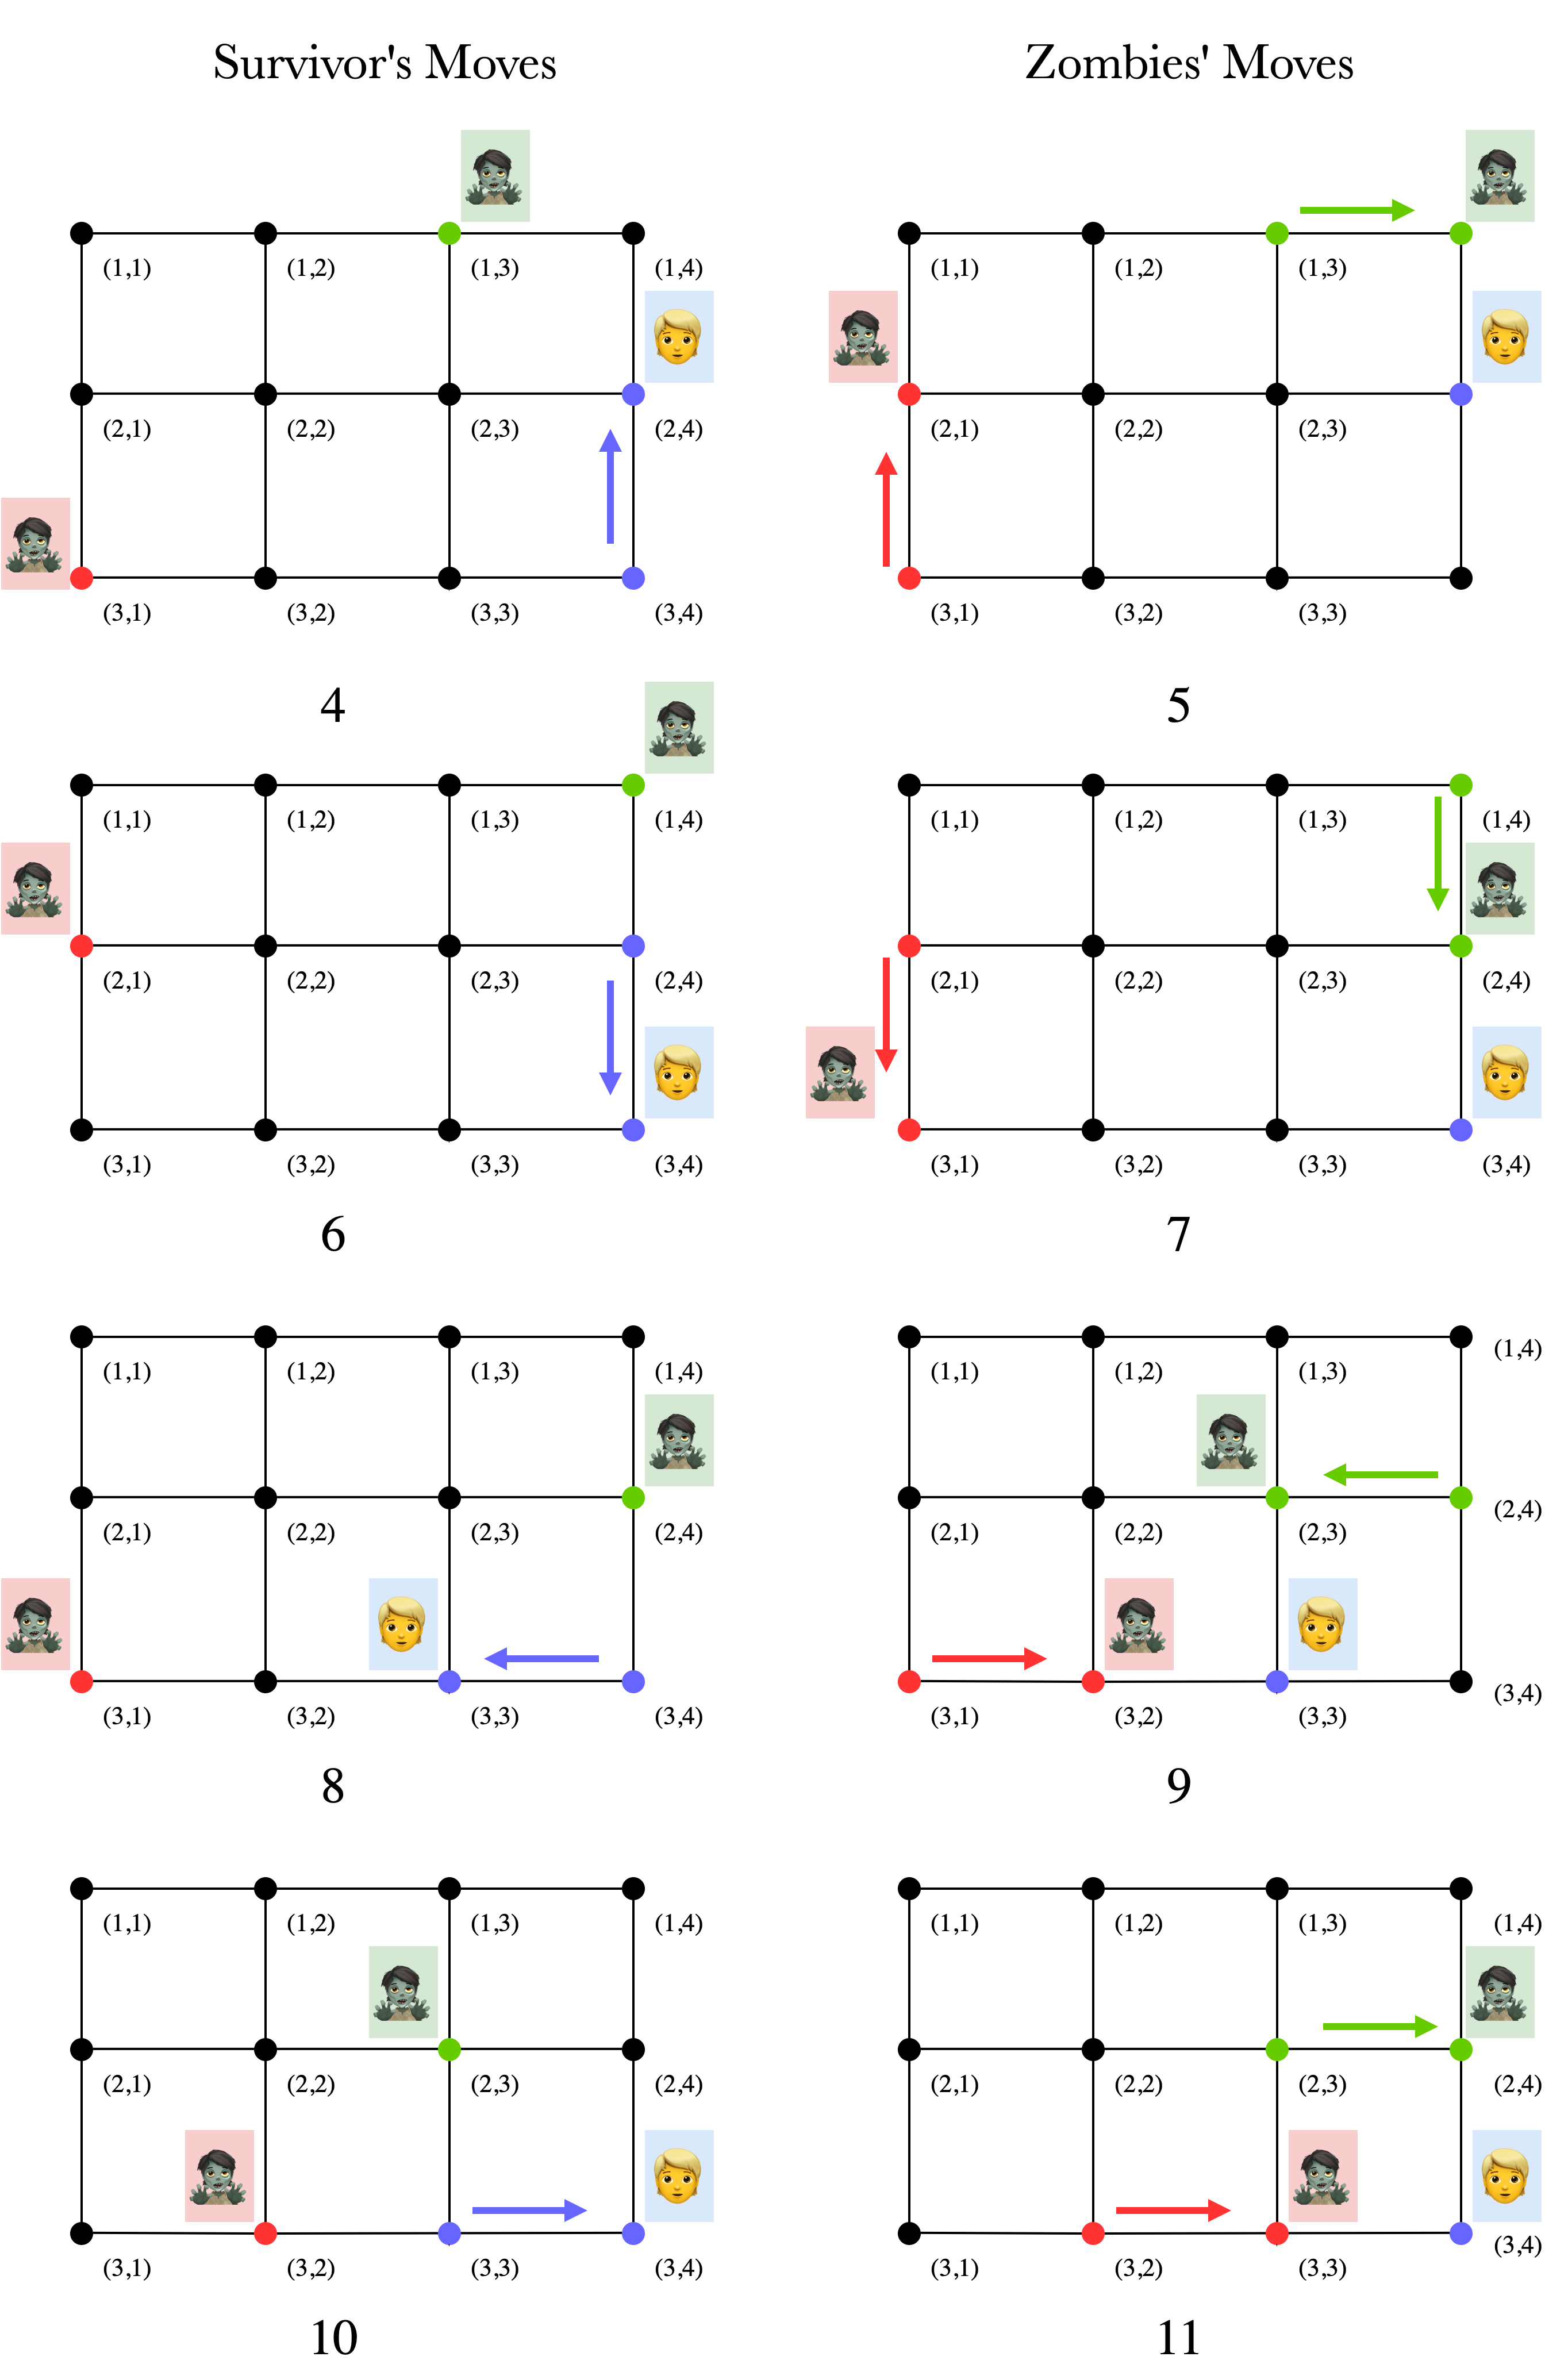
\includegraphics[width=0.6\linewidth]{fig/p34m6.png}
	\caption{Other moves made by players}
	\label{fig:p6}
\end{figure}

	
\end{document}